%%%%%%%%%%%%%%%%%%%%%%%% ExtendedAbstract.tex %%%%%%%%%%%%%%%%%%%%%%%%
%                                                                    %
%  Template for the 10-page extended abstract to be submitted for    %
%  the MSc degree conferral at Instituto Superior Tecnico.           %
%                                                                    %
%  Author:                                                           %
%                                                                    %
%       Andre C. Marta                                               %
%       Area Cientifica de Mecanica Aplicada e Aeroespacial          %
%       Departamento de Engenharia Mecanica                          %
%       Instituto Superior Tecnico                                   %
%       Av. Rovisco Pais                                             %
%       1049-001 Lisboa                                              %
%       Portugal                                                     %
%       Tel: +351 21 841 9466                                        %
%                        3466 (extension)                            %
%       Email: andre.marta@ist.utl.pt                                %
%                                                                    %
%  Created:       Dec  2, 2011                                       %
%  Last Modified: Dec 27, 2011                                       %
%%%%%%%%%%%%%%%%%%%%%%%%%%%%%%%%%%%%%%%%%%%%%%%%%%%%%%%%%%%%%%%%%%%%%%
% This document uses the LaTeX class file "article.cls"              %
%%%%%%%%%%%%%%%%%%%%%%%%%%%%%%%%%%%%%%%%%%%%%%%%%%%%%%%%%%%%%%%%%%%%%%
\documentclass[8pt,a4paper,twocolumn]{article}

%%%%%%%%%%%%%%%%%%%%%%%%%%%%%%%%%%%%%%%%%%%%%%%%%%%%%%%%%%%%%%%%%%%%%%
% Document preamble
%%%%%%%%%%%%%%%%%%%%%%%%%%%%%%%%%%%%%%%%%%%%%%%%%%%%%%%%%%%%%%%%%%%%%%

%% Builds upon the graphics  package, providing a key-value interface
%% for optional arguments to the \includegraphics command that go far
%% beyone what the graphics package offers.
%% http://www.ctan.org/tex-archive/help/Catalogue/entries/graphicx.html
%% if you use PostScript figures in your article
%% use the graphics package for simple commands
%% \usepackage{graphics}
%% or use the graphicx package for more complicated commands
%% \usepackage{graphicx}
%% or use the epsfig package if you prefer to use the old commands
%% \usepackage{epsfig}
\usepackage{graphicx} % Enhanced LaTeX Graphics
\usepackage{siunitx}

%Tipo de letra Arial
\usepackage{helvet}
\renewcommand{\familydefault}{\sfdefault}

% acentos e cedilhas
\usepackage[utf8]{inputenc}
%\usepackage[T1]{fontenc}

% Multiple figures
%\usepackage{subfigure} % subcaptions for subfigures
%\usepackage{subfigmat} % matrices of similar subfigures

\usepackage[font=footnotesize, skip = 1pt, labelfont=bf]{caption}
\usepackage[font=footnotesize]{subcaption}

% Declaring new column types
% 'dcolumn' package defines D to be a column specifier with
% three arguments: D{<sep.tex>}{<sep.dvi>}{<decimal places>}
%                  D{<sep.tex>}{<sep.dvi>}{<left digit places>.<right digit places>}
\usepackage{dcolumn}           % decimal-aligned tabular math columns
% d takes a single argument specifying the number of decimal places, e.g., d{2}
% or the number of digits to the left and right of the seperator, e.g., d{3.2}
\newcolumntype{.}   {D{.}{.}{-1}} % column alignedd on the point separator '.'
\newcolumntype{d}[1]{D{.}{.}{#1}} % column centered on the point separator '.'
\newcolumntype{e}   {D{E}{E}{-1}} % column centered on the exponent 'E'
\newcolumntype{E}[1]{D{E}{E}{#1}} % column centered on the exponent 'E'

%% American Mathematical Society (AMS) plain Tex macros
%%
%% The amsmath package is the principal package in the AMS-LaTeX distribution
%% http://www.ctan.org/tex-archive/help/Catalogue/entries/amsmath.html
\usepackage{amsmath}
\DeclareMathSizes{7}{7}{3}{3} 
\usepackage{pifont}
%%
%% The amsfonts package provides extended TeX fonts
%% http://www.ctan.org/tex-archive/help/Catalogue/entries/amsfonts.html
\usepackage{amsfonts}
%% The amssymb package provides various useful mathematical symbols
\usepackage{amssymb}
%%
%% The amsthm package provides extended theorem environments
%% http://www.ctan.org/tex-archive/help/Catalogue/entries/amsthm.html
\usepackage{amsthm}

%% Improves the interface for defining floating objects such as figures and tables.
%% The package also provides the H float modifier option of the obsolete here package.
%% http://www.ctan.org/tex-archive/help/Catalogue/entries/float.html
\usepackage{float}

%% Control sectional headers. 
%% http://www.ctan.org/tex-archive/help/Catalogue/entries/sectsty.html
\usepackage{sectsty}
%%
%% Redefine the font size of the 'section' and 'subsection' headings
\newcommand{\myFontSize}{\fontsize{9}{0}\selectfont}
\sectionfont{\myFontSize}       % 10pt, Bold face (default)
\subsectionfont{\myFontSize} % 10pt, Plain face

%% Select alternative section titles.
%% http://www.ctan.org/tex-archive/help/Catalogue/entries/titlesec.html
\usepackage{titlesec}
\usepackage{booktabs}
%\usepackage{multirow}
%\usepackage{array}
\usepackage{csquotes}% Recommended
%\usepackage[style=authoryear, backend=bibtex, doi=false,isbn=false,url=false,eprint=false,dashed=false,maxcitenames=2, maxbibnames=100]{biblatex}
%\addbibresource{library.bib}

%%
%% Left indent, before and after spacing
%% (The starred version kills the indentation of the paragraph following the title)
\titlespacing*{\section}{0pt}{10pt}{0pt}
\titlespacing*{\subsection}{0pt}{10pt}{0pt}

%% Section numbers with trailing dots. 
%% http://www.ctan.org/tex-archive/help/Catalogue/entries/secdot.html
\usepackage{secdot}
\usepackage{epstopdf}
%%
%% Also put a dot after the subsection number
\sectiondot{subsection}
%% Set a space between dot and heading text
\sectionpunct{section}{. }    % By default, \sectiondot places a \quad
\sectionpunct{subsection}{. } % after the number

% These are exact settings for a A4 page with top margin of
% 25 mm, bottom margin of 30 mm, left and right margins of 25 mm,
% printable area 242 X 160 mm.

\setlength{\topmargin}{-10.4mm}
\setlength{\headheight}{0.0mm}
\setlength{\headsep}{10.0mm}
\setlength{\textwidth}{160mm}
\setlength{\textheight}{242mm}
\setlength{\oddsidemargin}{0mm}
\setlength{\evensidemargin}{0mm}
\setlength{\marginparwidth}{0mm}
\setlength{\marginparsep}{0mm}

% New command to refer to equations as Eq.(1),Eq.(2),...
\newcommand{\eqnref}[1]{Eq.(\ref{#1})}

%%%%%%%%%%%%%%%%%%%%%%%%%%%%%%%%%%%%%%%%%%%%%%%%%%%%%%%%%%%%%%%%%%%%%%%%%%%%%%%%%%%%%%%%
% Title, authors and addresses

\title{\bfseries Evaluation of the Effectiveness of Packet Erasure Codes in a Docker-Simulated Network}
\date{Apr 2024}
\author{Chan Ming Han \\ Ng Mu Rong \\  Pei Xin \\ \\ University of California, Berkeley}

%%%%%%%%%%%%%%%%%%%%%%%%%%%%%%%%%%%%%%%%%%%%%%%%%%%%%%%%%%%%%%%%%%%%%%%%%%%%%%%%%%%%%%%%
\begin{document}

% Begin one column section for title and abstract
%
% http://www.faqs.org/faqs/de-tex-faq/part5/
\twocolumn[
\begin{@twocolumnfalse}
\maketitle

	%%%%%%%%%%%%%%%%%%%%%%%%%%%%%%%%%%%%%%%%%%%%%%%%%%%%%%%%%%%%%%%%%%%%%%
%     File: ExtendedAbstract_abstr.tex                               %
%     Tex Master: ExtendedAbstract.tex                               %
%                                                                    %
%     Author: Andre Calado Marta                                     %
%     Last modified : 2 Dez 2011                                     %
%%%%%%%%%%%%%%%%%%%%%%%%%%%%%%%%%%%%%%%%%%%%%%%%%%%%%%%%%%%%%%%%%%%%%%
% The abstract of should have less than 500 words.
% The keywords should be typed here (three to five keywords).
%%%%%%%%%%%%%%%%%%%%%%%%%%%%%%%%%%%%%%%%%%%%%%%%%%%%%%%%%%%%%%%%%%%%%%

%%
%% Abstract
%%
\begin{abstract}
    THIS IS THE ABSTTRACT
    \\
    %%
    %% Keywords (max 5)
    %%
    \noindent{{\bf Keywords:}} Packet Erasure Codes, Network Simulation \\
    
    \end{abstract}
    
    

\end{@twocolumnfalse}
]
	\section{Background}
\label{sec:background}

Erasure coding is a method of data protection by which data is 
broken into packets. These packets are then expanded and encoded 
with redundant data pieces so that the original data is still preserved 
in case of packet erasure or outages. In the context of communication 
networks, packet erasure coding \cite{WalrandParekh2017} is used in the case of multicasting, 
where it is infeasible for the source node to track acknowledgements from 
all the destination nodes. As such, this scheme is designed to be able to 
recover from the “erasures”, or dropping of packets as packets propagate 
through the network.
	% A Theory section should extend, not repeat, the background to the
% article already dealt with in the Introduction and lay the
% foundation for further work.

\section{Introduction}
\label{sec: backg}

Lorem ipsum dolor sit amet, consectetur adipiscing elit, sed do eiusmod tempor incididunt ut labore et dolore magna aliqua. Ut enim ad minim veniam, quis nostrud exercitation ullamco laboris nisi ut aliquip ex ea commodo consequat. Duis aute irure dolor in reprehenderit in voluptate velit esse cillum dolore eu fugiat nulla pariatur. Excepteur sint occaecat cupidatat non proident, sunt in culpa qui officia deserunt mollit anim id est laborum.

Lorem ipsum dolor sit amet, consectetur adipiscing elit, sed do eiusmod tempor incididunt ut labore et dolore magna aliqua. Ut enim ad minim veniam, quis nostrud exercitation ullamco laboris nisi ut aliquip ex ea commodo consequat. Duis aute irure dolor in reprehenderit in voluptate velit esse cillum dolore eu fugiat nulla pariatur. Excepteur sint occaecat cupidatat non proident, sunt in culpa qui officia deserunt mollit anim id est laborum.


\begin{table*}[!htbp]
	\footnotesize
	\centering
	\caption{Comparative analysis of drug administration routes}
	\label{tbl: 1.1a}
	\renewcommand{\arraystretch}{0.8}
	\begin{tabular}{@{}lllll@{}}
		\toprule[1pt]
		&  & \textbf{Advantages}     & \textbf{} & \textbf{Disadvantages}                                                                                             \\ \midrule
		%&&&&\\
		\textbf{Oral}       &  & Convenient              &           & Highly variable absorption time                                                                                    \\
		&  & Inexpensive             &           & Systemic side affects (e.g.\ First pass metabolism)                                                                 \\
		&  & Portable                &           & Drug may be inactivated (e.g.\ Food ingested)                                                                       \\
		&  &                         &           &                                                                                                                    \\
		\textbf{Injection}  &  & Bioavailability (100\%) &           & Special equipment and trained personnel required                                                                   \\
		&  & Fastest onset of action &           & Expensive (Transportation and storage costs)                                                                                \\
		&  &                         &           & Invasive, can cause injuries and disease \\
		&  &                         &           & transmission (e.g.\ Embolism, Phlebitis)                                                                                                                   \\
		&  &                         &           &                                                                                                                    \\
		\textbf{Inhalation} &  &  On-target delivery (Lung related diseases)             &           & Irritation of the respiratory tract may take place                                               \\
		&  & Rapid onset of action   &           &  Variable dosing (e.g.\ Faulty inhalation technique                                                                                                                        \\
		&  & Low drug dosage       &          &   Special apparatus is required                                                                                                                \\ \bottomrule[1pt]
		%&  &                         &           &                                                                                                                    \\ \bottomrule[1pt]
	\end{tabular}
\end{table*}




	\section{Methodology}
\label{sec: Methodology}

The idea of this project was to vary the values of $\it{redundancyFactor}$ and $\it{packetDropRate}$, and finally determine the probability that a receiver can accurately decode a message. \\
With these definitions, we have: 
\begin{equation} \label{eq: yPlus}
    m = \rho_{rf} \cdot k
\end{equation}

where $\rho_{rf}$ is the $\it{redundancyFactor}$, $k$ is the number of original packets after packetizing a stream, and $m$ is the total number of packets to be sent through the network. This provides us 
$m-n$ redundant packets in the network. Based on the $zfec$ encoder, a receiver would be able to decode the message as long as it received any $n$ of the $m$ messasges in the network. The value of $\rho_{rf}$ was then varied, $0\leq\rho_{rf}\leq1$. It should be noted that when $\rho_{rf} = 0$, this degenerates to sending the raw packets over the network, with no redundancy. \\
Next, we also varied the value of $packetDropRate$, where all routers in the network had a specific constant $\omega$. This was key to emulating the idea of an unrealiable network. 

\begin{equation} \label{eq: yPlus}
    P(routerForward) = 1-\omega
\end{equation}


\subsection{Topology Generation}

To setup the network in the docker environment, we decided to employ the use of an
Erdos-Renyi graph.
In the context of emulating a router network for a networks project, employing the Erdős-Rényi (E-R) model is particularly advantageous due to its fundamental characteristics, which mirror aspects of the real-world structure of the Internet\cite{Li2021}. The Erdős-Rényi graph is a type of random graph where edges between pairs of nodes are established with a constant probability, independent of other edges. This stochastic nature of the E-R model captures the inherent randomness and organic development observed in the topology of the World Wide Web. Unlike more deterministic models or regular graphs where the connections are fixed and predictable, the E-R model allows for the exploration of network behaviors under various random configurations, reflecting the unpredictable nature of real-world networks. This aspect is crucial for studying properties such as network robustness, connectivity, and path diversity, which are integral to understanding and designing efficient and resilient router networks. The flexibility and simplicity of the E-R graph make it a suitable choice for modeling networks that need to represent a wide array of potential connection scenarios, akin to the complex and diverse linkage seen in the global Internet infrastructure.

\subsection{Simulation Parameters}

To simulate the experiment, we created a network of 20 nodes using python's networkx, with $p=0.2$, where $p$ represents the probability of edge creation. We also attached a host to each of these routers, where a random selected host was to be our
final $receiver$ node (acting as the unicast receiver), which decodes the transmitted packets. 
In each experiment, a total of 
200 different messages were sent, each of 200 words long. 



\subsection{Encoding and Decoding}
The encoding and decoding scheme is implemented by the zfec library \cite{Rizzo2013}.
The encoding is parameterized by two integers, k and m. m is the total number of blocks produced, and k is how many of those blocks are necessary to reconstruct the original data.
Data is divided into "primary blocks" sized at $\frac{1}{k}$ of the original data.
"Secondary blocks" are generated on primary blocks for redundancy.
Metadata, including $k$, $m$, share numbers, and padding, is generated. 
The metadata and blocks are then compressed and appended to each share.
The final encoded data comprises $m$ blocks, each containing compressed metadata and data blocks.
The decoding process is the reverse of encoding.
Minimum $k$ blocks are required for decoding.
Compressed metadata is extracted and decompressed to retrieve necessary information.
The original data is then reconstructed using metadata and selected blocks.




% \begin{equation} \label{eq: yPlus}
% y^+ = \frac{u_\tau y}{\nu} = \frac{y}{\nu}\sqrt{\frac{\tau_\omega}{\rho}}
% \end{equation}

% Lorem ipsum dolor sit amet, consectetur adipiscing elit, sed do eiusmod tempor incididunt ut labore et dolore magna aliqua. Ut enim ad minim veniam, quis nostrud exercitation ullamco laboris nisi ut aliquip ex ea commodo consequat. Duis aute irure dolor in reprehenderit in voluptate velit esse cillum dolore eu fugiat nulla pariatur. Excepteur sint occaecat cupidatat non proident, sunt in culpa qui officia deserunt mollit anim id est laborum.
% \begin{equation} \label{eq: Shear Stress at the Wall}
% \tau_{\omega} = \frac{1}{2} \rho C_f U^2
% \end{equation}

% Lorem ipsum dolor sit amet, consectetur adipiscing elit, sed do eiusmod tempor incididunt ut labore et dolore magna aliqua. Ut enim ad minim veniam, quis nostrud exercitation ullamco laboris nisi ut aliquip ex ea commodo consequat. Duis aute irure dolor in reprehenderit in voluptate velit esse cillum dolore eu fugiat nulla pariatur. Excepteur sint occaecat cupidatat non proident, sunt in culpa qui officia deserunt mollit anim id est laborum.

% \begin{equation} \label{eq: yPlus development}
% y^+ = \frac{y}{\nu}\sqrt{\frac{\frac{1}{2}\rho C_f U^2}{\rho}} = \underbrace{\left(\frac{UD}{\nu}\right)}_{Re_{D}}\frac{y}{D}\sqrt{\frac{C_f}{2}}
% \end{equation}

	\section{Results \& discussion}
\label{sec:resul}
Due to each run of the experiment needing to spin up 30 docker containers and run Link State Protocol to convergence to generate routing tables,
each simulation took a lot of compute and ran for approximately 3 minutes. As such, the experimental surface plot was smoothened using a linear interpolating technique
to generate more plot points. Also, each experiment was only run once per setting of redundancy factor and packet drop rate, and further, due to randomness in graph generation, there are some 
outliers in the graph. 

\begin{figure}[ht]
    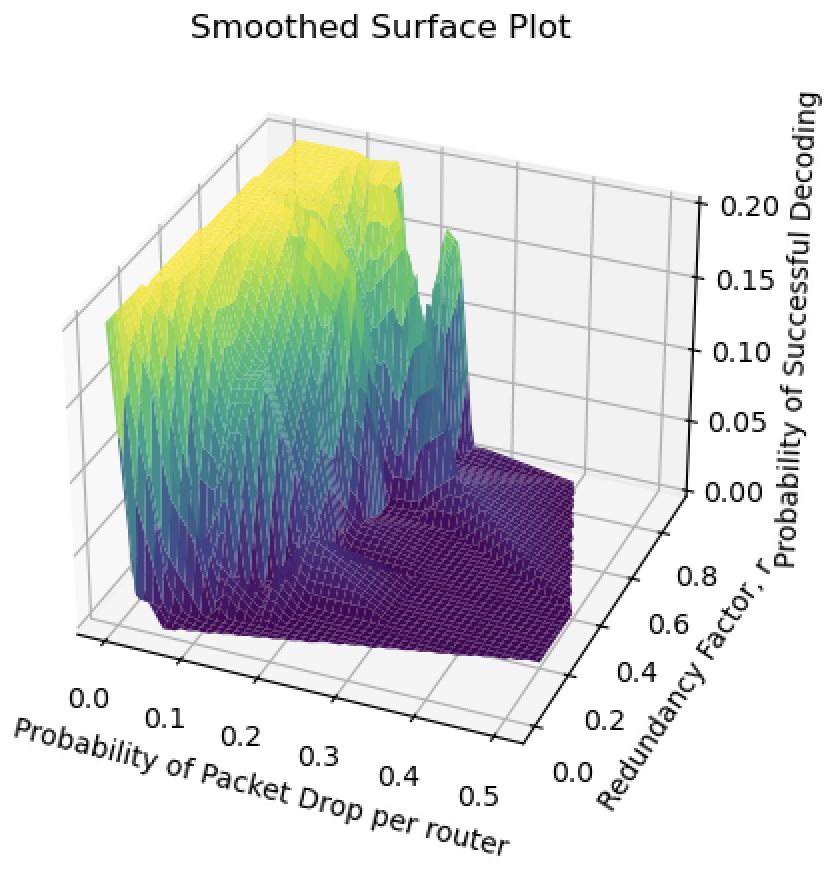
\includegraphics[width=0.48\textwidth]{experimental.png}  % Replace 'filename.ext' with your image file.
    \caption{Experimental Surface Plot=}  % Optional: add a caption.
\end{figure}

Nonetheless, we see that our surface plot roughly resembles the theoretical surface plot. We find that further work can be done to analyse the 
maximum of these surface plots, and a unconstrained optimization technique could be used to find the most suitable redundancy factor based on the unreliability of the particular network 
that a payload is about to be transferred over. 


\subsection{Theoretical Analysis}
Assuming that every router in the network has the same packet drop rate, we arrive at the following equations.
\begin{equation} \label{eq: yPlus}
    N = (1+\rho_{rf})*n
\end{equation}
where $N$ is the effective number of packets.
Further, defining $s$ as the survival per hop, we have 

\begin{equation} \label{eq: yPlus}
    s = 1-\omega
\end{equation}
In order for a packet to survive all hops, we have 
\begin{equation} \label{eq: yPlus}
    s_a = s^{h}
\end{equation}
where $h$ is the average number of hops taken by the packet thorugh the network. As such, we arrive at a final probability $p$ \\

\begin{equation} \label{eq: yPlus}
    p = \sum_{k=n}^{N}{N\choose k}s_a^k(1-s_a)^{N-k}
\end{equation}

Using this equation, we are able to plot the theoretical surface plot as shown.

\begin{figure}[ht]
    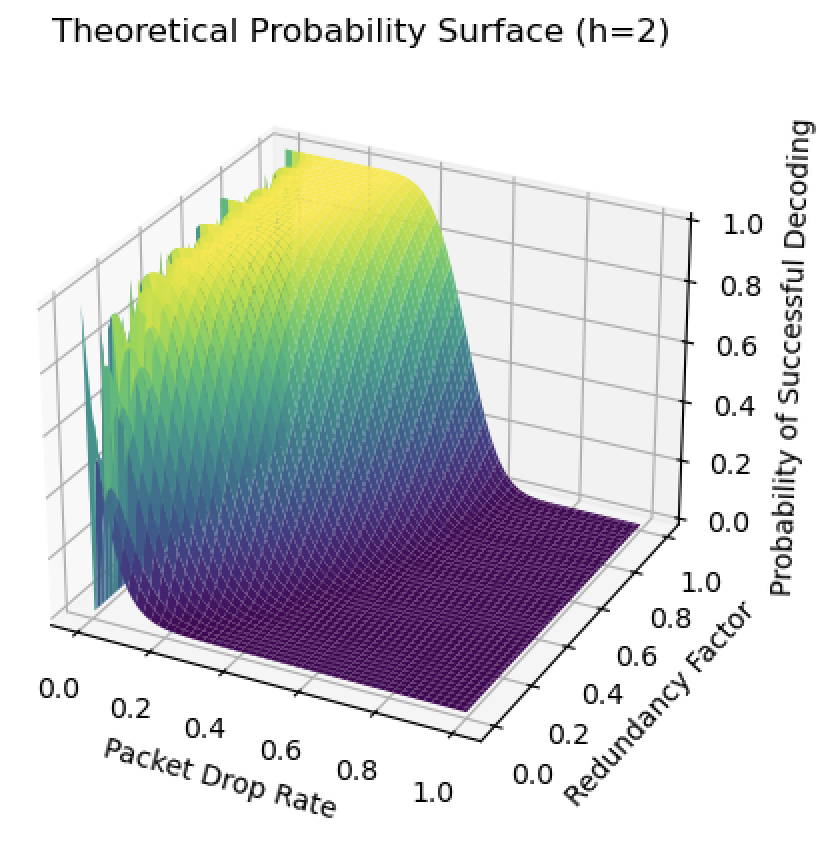
\includegraphics[width=0.48\textwidth]{2hops.png}  % Replace 'filename.ext' with your image file.
    \caption{Theoretical Surface Plot with h-2}  % Optional: add a caption.
\end{figure}

As we can see from the theoretical plot, as packet drop rate increases, the probability of a successful decoding decreases exponentially. 
This "unreliability" in the network can be offset by sending redundant packets as seen by the yellow surface in the plot. However, this only works to a certain extent, and when 
packet drop rates beyond 0.5 still result in a very low probability of successful decoding. It should also be noted that with larger payloads, the probability of a successful decoding could
be much lower. 





	\section{Conclusions}
\label{sec:concl}

Lorem ipsum dolor sit amet, consectetur adipiscing elit, sed do eiusmod tempor incididunt ut labore et dolore magna aliqua. Ut enim ad minim veniam, quis nostrud exercitation ullamco laboris nisi ut aliquip ex ea commodo consequat. Duis aute irure dolor in reprehenderit in voluptate velit esse cillum dolore eu fugiat nulla pariatur. Excepteur sint occaecat cupidatat non proident, sunt in culpa qui officia deserunt mollit anim id est laborum.

Lorem ipsum dolor sit amet, consectetur adipiscing elit, sed do eiusmod tempor incididunt ut labore et dolore magna aliqua. Ut enim ad minim veniam, quis nostrud exercitation ullamco laboris nisi ut aliquip ex ea commodo consequat. Duis aute irure dolor in reprehenderit in voluptate velit esse cillum dolore eu fugiat nulla pariatur. Excepteur sint occaecat cupidatat non proident, sunt in culpa qui officia deserunt mollit anim id est laborum.

Lorem ipsum dolor sit amet, consectetur adipiscing elit, sed do eiusmod tempor incididunt ut labore et dolore magna aliqua. Ut enim ad minim veniam, quis nostrud exercitation ullamco laboris nisi ut aliquip ex ea commodo consequat. Duis aute irure dolor in reprehenderit in voluptate velit esse cillum dolore eu fugiat nulla pariatur. Excepteur sint occaecat cupidatat non proident, sunt in culpa qui officia deserunt mollit anim id est laborum.

Lorem ipsum dolor sit amet, consectetur adipiscing elit, sed do eiusmod tempor incididunt ut labore et dolore magna aliqua. Ut enim ad minim veniam, quis nostrud exercitation ullamco laboris nisi ut aliquip ex ea commodo consequat. Duis aute irure dolor in reprehenderit in voluptate velit esse cillum dolore eu fugiat nulla pariatur. Excepteur sint occaecat cupidatat non proident, sunt in culpa qui officia deserunt mollit anim id est laborum.

% REFERENCES

% Produces the bibliography section when processed by BibTeX
%
% Bibliography style
% > entries ordered alphabetically
%\bibliographystyle{plain}
% > unsorted with entries appearing in the order in which the citations appear.
%\bibliographystyle{unsrt}
% > entries ordered alphabetically, with first names and names of journals and months abbreviated
\bibliographystyle{abbrv}
% > entries ordered alphabetically, with reference markers based on authors' initials and publication year
%\bibliographystyle{alpha}

% External bibliography database file in the BibTeX format (ExtendedAbstract_ref_db.bib)
\bibliography{references}

\end{document}


